\section{Solarzelle}

\subsection{Aufbau Solarzelle}

\begin{center}
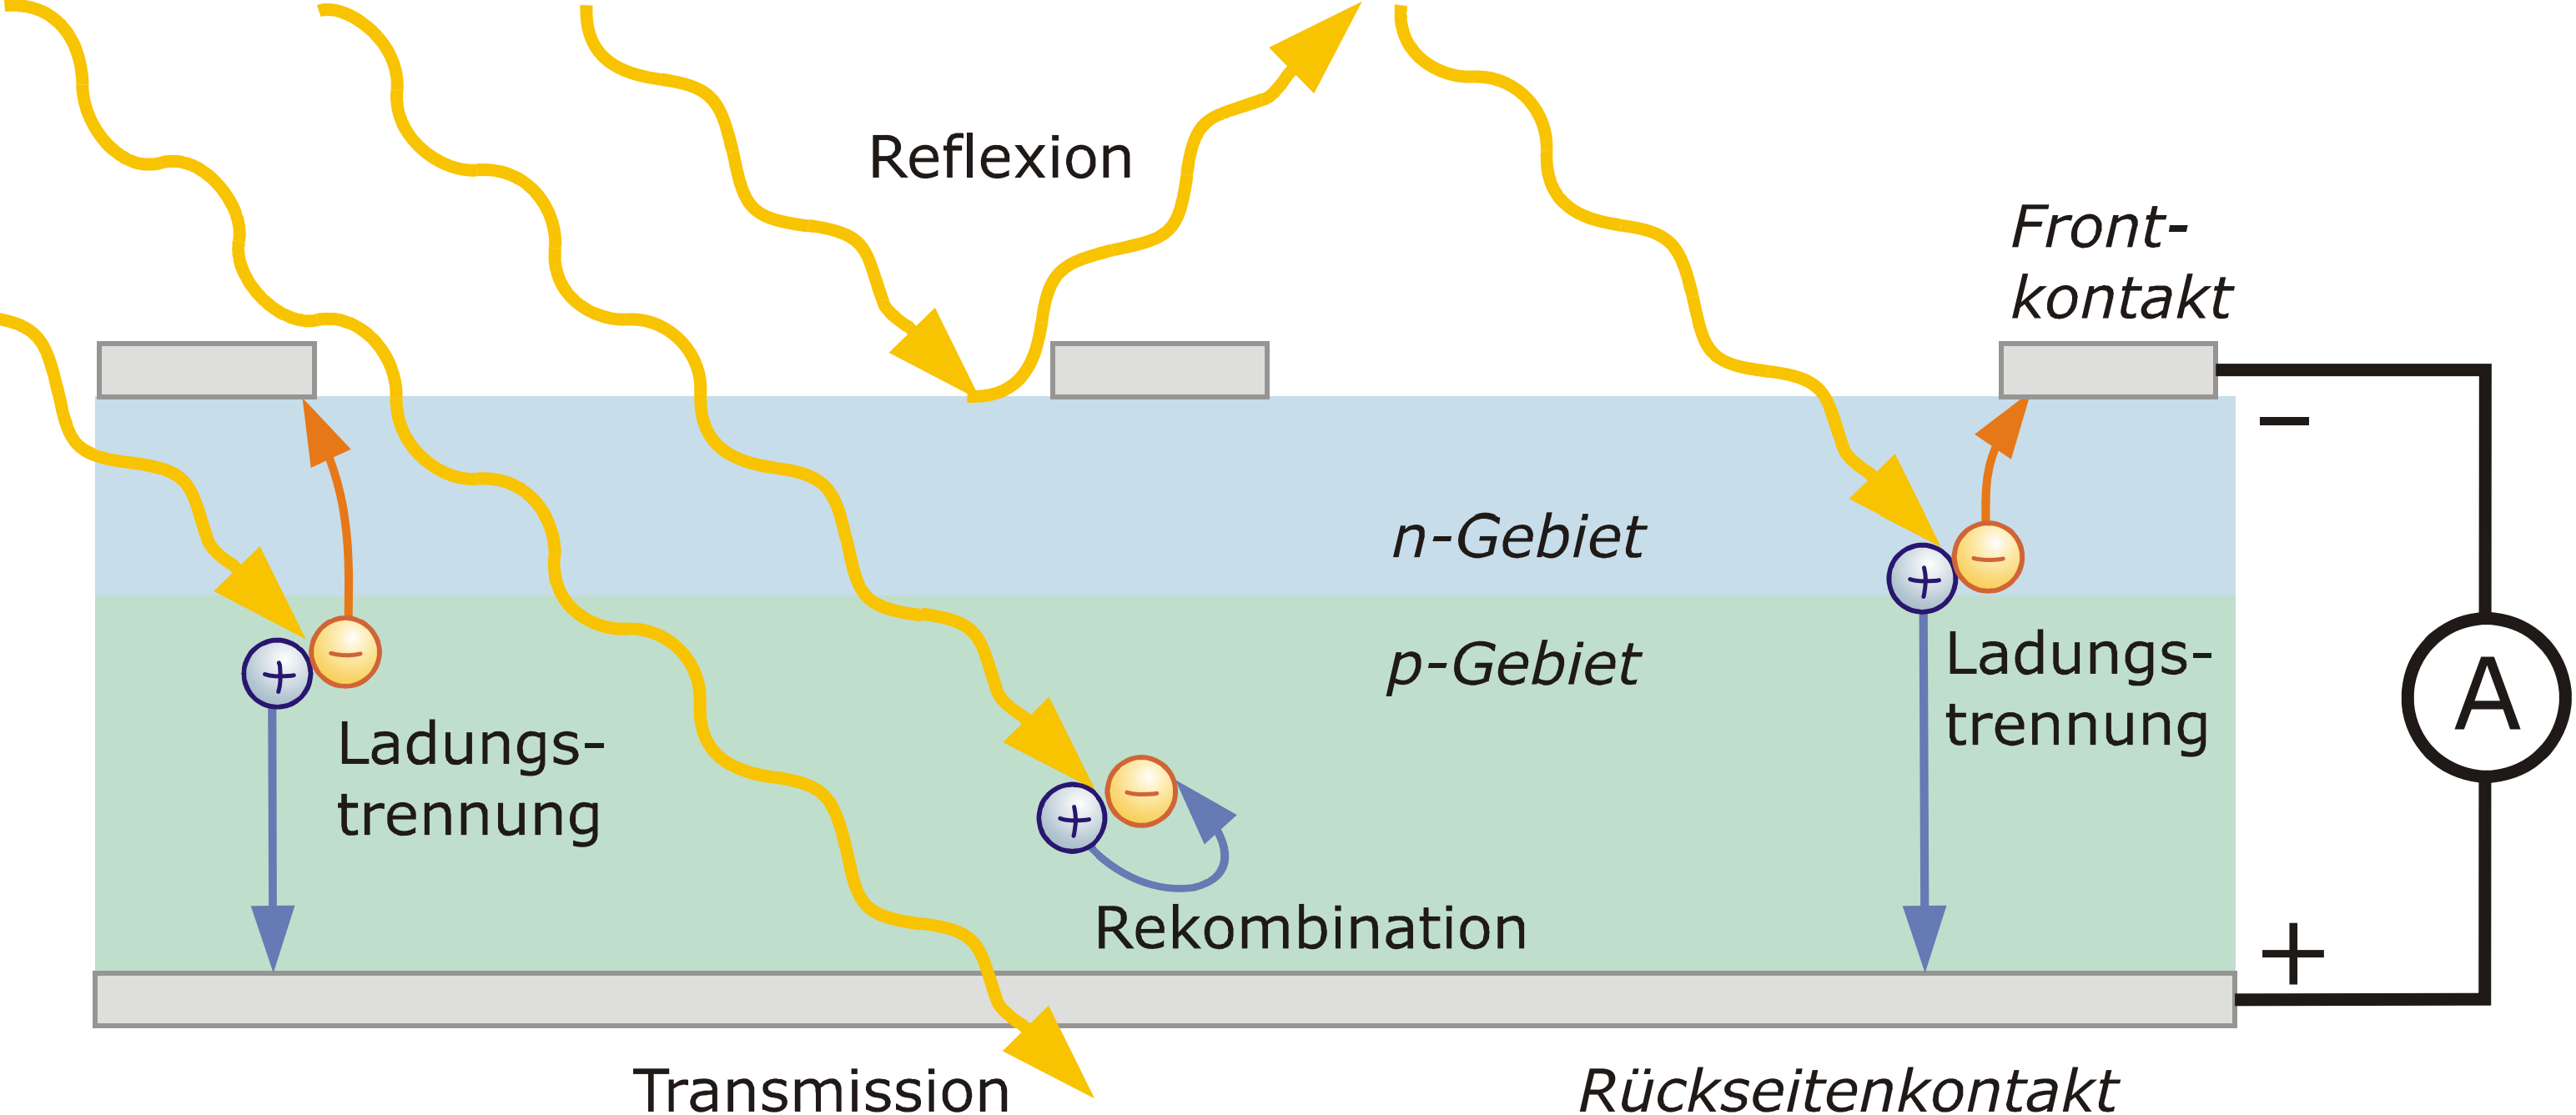
\includegraphics[width=0.8\linewidth]{images/Solarzelle_bei_Bestrahlung.png}
\end{center}

%\begin{center}
%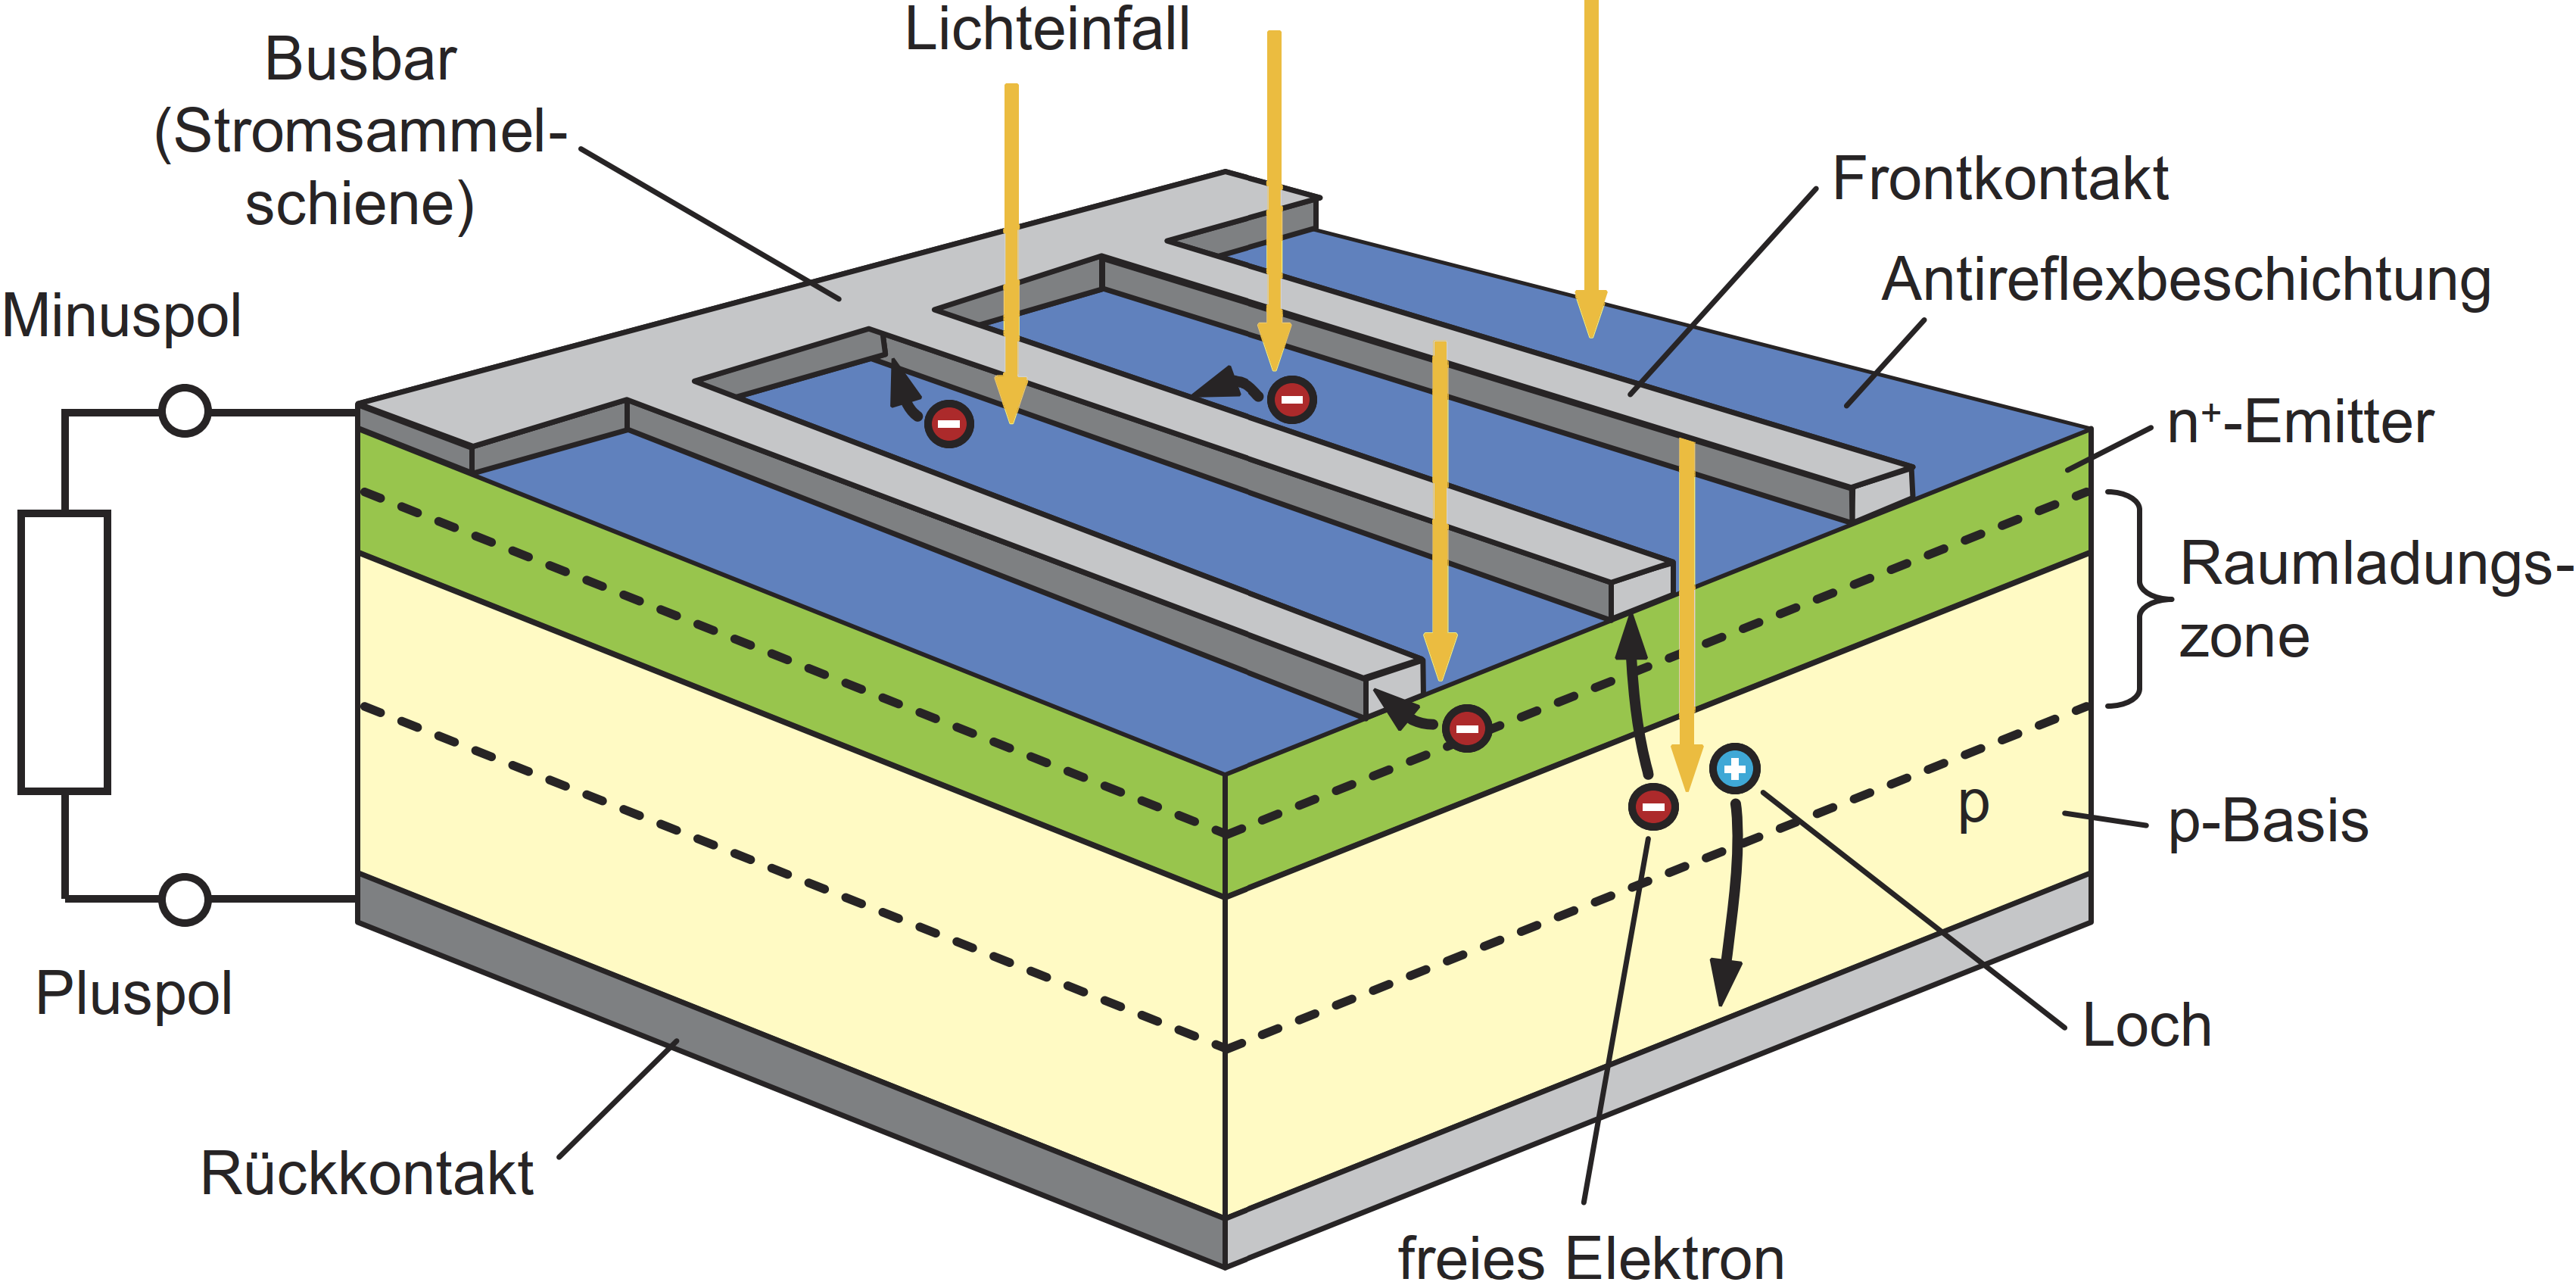
\includegraphics[width=0.9\linewidth]{images/Aufbau_Solarzelle.png}
%\end{center}

\subsection{Reflexionsfaktor}

\begin{minipage}[c]{0.2\columnwidth}
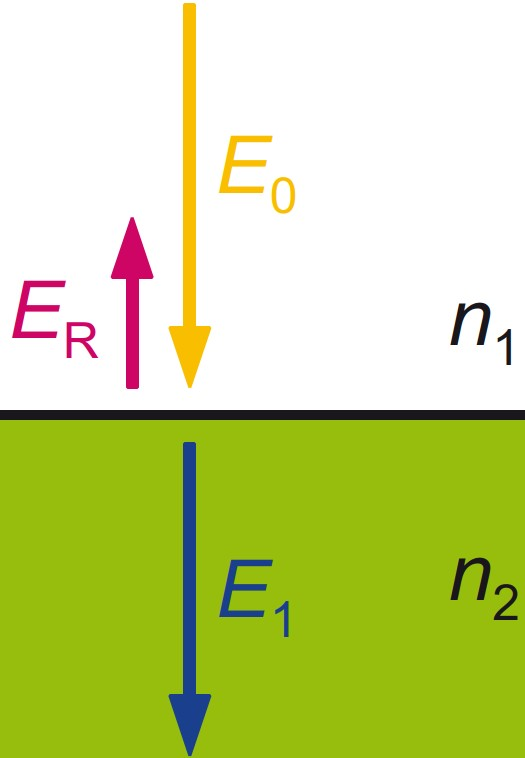
\includegraphics[width=0.98\linewidth]{images/Regflexion.jpg}
\end{minipage}
\hfill
\begin{minipage}[c]{0.78\columnwidth}

    $\boxed{R=\left (\frac{n_1-n_2}{n_1+n_2}\right)^2}
    \quad
    \boxed{R = \frac{E_{\mathrm{R}}}{E_{\mathrm{0}}}}
    $

    \vspace{0.1cm}

    \renewcommand{\arraystretch}{1.2}
    \begin{tabular}{@{} l p{5.5cm} l @{}}
        $[R]$                   & Reflexionsfaktor  \dotfill & $\mathrm{-}$ \\
        $[n_1]$                 & Brechungsindex 1 (Luft = 1)  \dotfill & $\mathrm{-}$ \\
        $[n_2]$                 & Brechungsindex 2  \dotfill & $\mathrm{-}$ \\
        $[E_{\mathrm{0}}]$      & Einfallende Strahlungsstärke  \dotfill & $\frac{\mathrm{W}}{\mathrm{m^2}}$\\
        $[E_{\mathrm{R}}]$      & Reflektierte Strahlungsstärke \dotfill & $\frac{\mathrm{W}}{\mathrm{m^2}}$
    \end{tabular}
\end{minipage}




\subsection{Quantenwirkungsgrad}



\subsubsection{Externer Quantenwirkungsgrad $\eta_{\mathrm{Ext}}$}

Nicht alle erzeugten Elektron-Loch-Paare tragen zum Photostrom bei. Daher definiert man den externen Quantenwirkungsgrad \( \eta_\text{Ext} \) als das Verhältnis der für den Photostrom nutzbaren Elektron-Loch-Paare zu den insgesamt auftreffenden Photonen.

\vspace{0.1cm}

\begin{minipage}[t]{0.2\columnwidth}
$
\boxed{\eta_{\text{Ext}} = \frac{N_{ELP}}{N_{Ph}}}
$
\end{minipage}
\hfill
\begin{minipage}[t]{0.78\columnwidth}
    \renewcommand{\arraystretch}{1.2}
\begin{tabular}{@{} l p{5.5cm} l @{}}
    $[\eta_{\mathrm{Ext}}]$   & Externer Quantenwirkungsgrad  \dotfill & $\mathrm{-}$ \\
    $[N_{\mathrm{ELP}}]$    & Anzahl nutzbarer Elektronen-Loch-Paare        \dotfill & $\mathrm{-}$ \\
    $[N_{\mathrm{Ph}}]$       & Anzahl auftretender Photonen  \dotfill & $\mathrm{-}$ \\
\end{tabular}
\end{minipage}


\subsubsection{Interner Quantenwirkungsgrad $\eta_{\mathrm{Int}}$}

Neben dem externen definiert man auch den internen Quantenwirkungsgrad \( \eta_\text{Int} \), bei dem die durch Reflexion verursachten Verluste herausgerechnet werden.

\vspace{0.1cm}


\begin{minipage}[t]{0.2\columnwidth}
$
\boxed{\eta_{\text{Int}} = \frac{\eta_{\text{Ext}}}{1 - R}}
$
\end{minipage}
\hfill
\begin{minipage}[t]{0.78\columnwidth}
    \renewcommand{\arraystretch}{1.2}
\begin{tabular}{@{} l p{5.5cm} l @{}}
    $[\eta_{\mathrm{Int}}]$   & Interner Quantenwirkungsgrad  \dotfill & $\mathrm{-}$ \\
    $[\eta_{\mathrm{Ext}}]$   & Externer Quantenwirkungsgrad  \dotfill & $\mathrm{-}$ \\
    $[R]$                     & Reflexionsfaktor  \dotfill & $\mathrm{-}$ \\
\end{tabular}
\end{minipage}



\subsection{Rekombination}

Rekombination bezeichnet den Prozess, bei dem Elektronen und Löcher in einem Halbleiter wieder zusammenfinden und dabei ihre Energie abgeben. Dies kann durch Wärme oder Lichtemission geschehen.

\vspace{0.1cm}

\begin{itemize}
  \item Störstellenrekombination an Fremdatomen oder Kristallfehlern
  \item Oberflächenrekombination
\end{itemize}

\vspace{0.1cm}

\textbf{Diffusionslänge} \( L_N \) Silizium: 50 -- 500\,µm



\subsection{Lichtabsorbtion, Bestrahlungsstärke und Eindringtiefe}

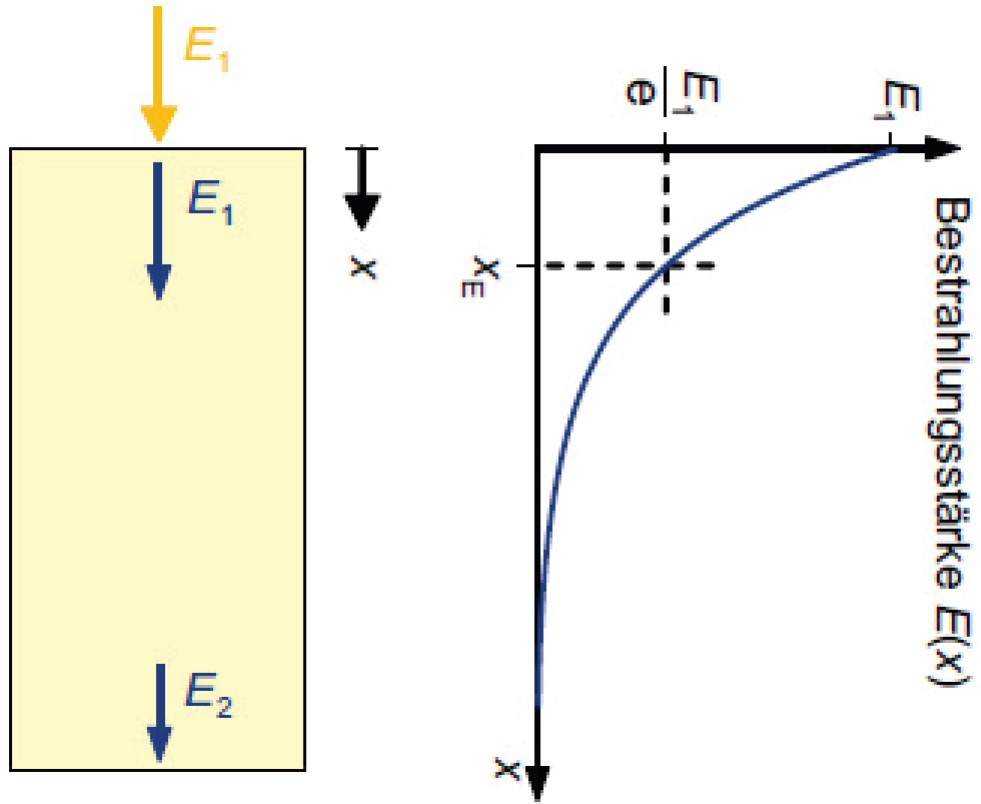
\includegraphics[width=0.6\linewidth]{images/Lichtabsorption.jpg}

\vspace{0.1cm}

$
\boxed{
E(x) = E_1 \cdot e^{-\alpha \cdot x}
}
\quad
\boxed{
x_\mathrm{E} = \frac{1}{\alpha}
}
$

\vspace{0.1cm}

\renewcommand{\arraystretch}{1.2}
\begin{tabular}{@{} l p{6.5cm} l @{}}
    $[E(x)]$      & Bestrahlungsstärke in Tiefe $x$ \dotfill & $\frac{\mathrm{W}}{\mathrm{m^2}}$ \\
    $[E_1]$       & Bestrahlungsstärke an der Oberfläche ($x=0$) \dotfill & $\frac{\mathrm{W}}{\mathrm{m^2}}$ \\
    $[\alpha]$    & Absorptionskoeffizient \dotfill & $\frac{\mathrm{1}}{\mathrm{m}}$ \\
    $[x]$         & Eindringtiefe \dotfill & $\mathrm{m}$ \\
    $[x_\mathrm{E}]$ & Eindringtiefe des Lichts \dotfill & $\mathrm{m}$ \\
\end{tabular}


\subsection{Absorptionswirkungsgrad}

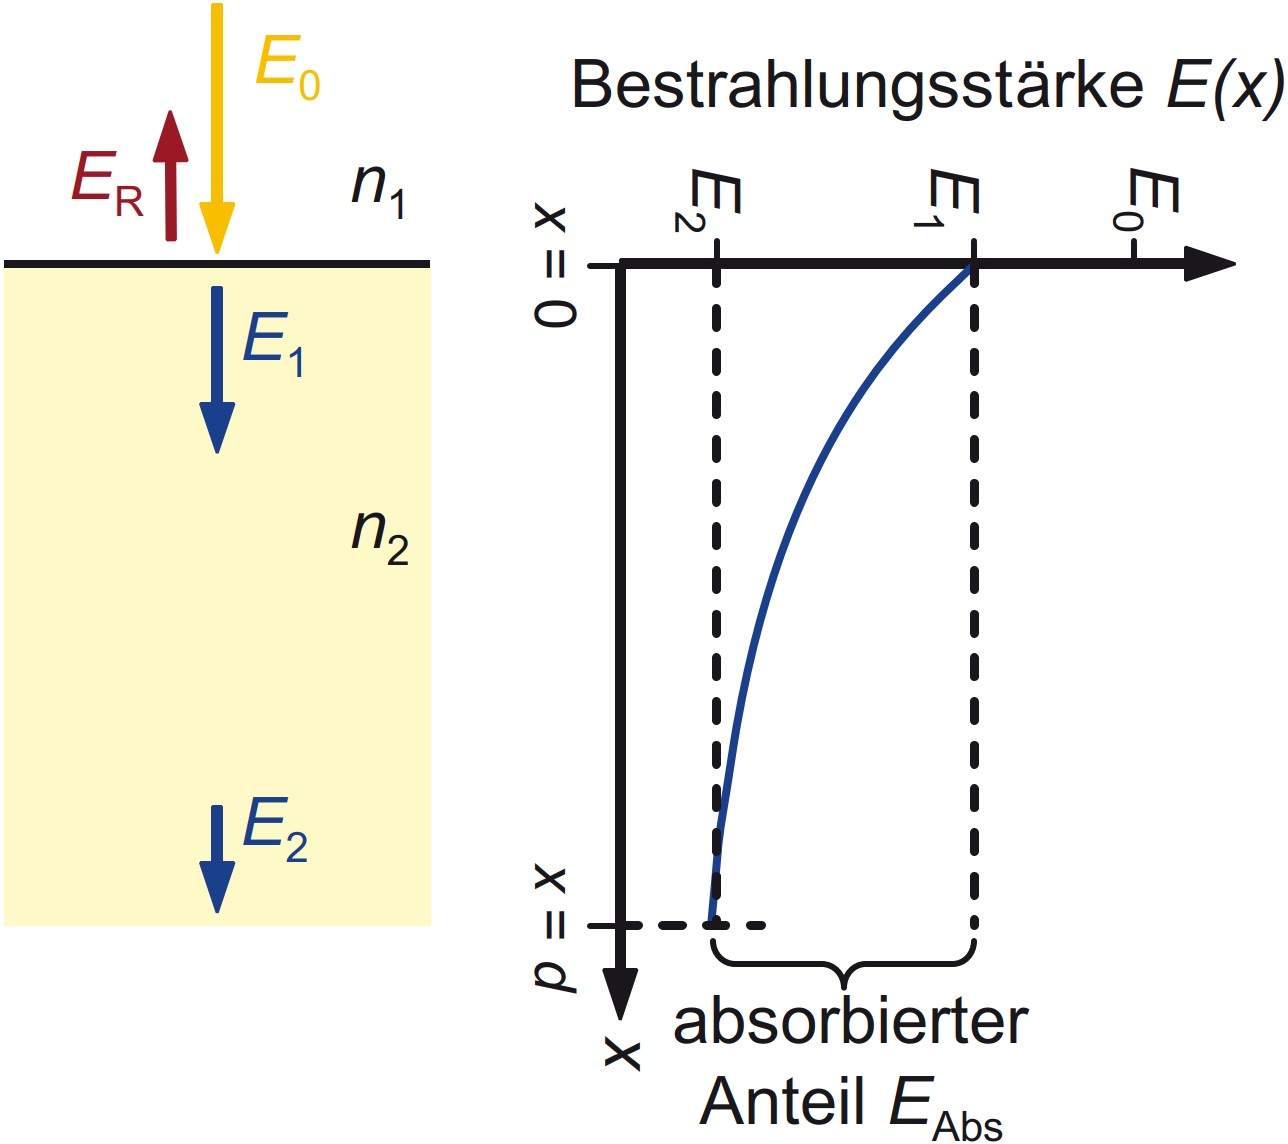
\includegraphics[width=0.6\linewidth]{images/Absorptionswirkungsgrad.jpg}

\vspace{0.1cm}

Wir definieren den Absorptionswirkungsgrad $\eta_\mathrm{Abs}$ als das Verhältnis der Zahl der absorbierten Photonen zur Zahl der aussen auftreffenden Photonen:

\vspace{0.1cm}

$
\boxed{
\eta_\mathrm{Abs} = \frac{N_\mathrm{Ph\_Abs}}{N_\mathrm{Ph}}
}
$
$
\boxed{
\eta_\mathrm{Abs} =  \frac{E_\mathrm{Abs}}{E_0}
}
$
$
\boxed{
\eta_\mathrm{Abs}  \frac{E_1 - E_2}{E_0}
}
$
$
\boxed{
\eta_\mathrm{Abs} = (1 - R) \cdot \left(1 - \mathrm{e}^{-\alpha \cdot d} \right)
}
$

$
\boxed{
E_{1} = (1 - R) \cdot E_0
}
$
$
\boxed{
E_{2} = E_1 \cdot e^{- \alpha \cdot d}
}
$

\vspace{0.1cm}

\renewcommand{\arraystretch}{1.2}
\begin{tabular}{@{} l p{6.5cm} l @{}}
    $[\eta_{\mathrm{Abs}}]$   & Absorptionswirkungsgrad  \dotfill & $\mathrm{-}$ \\
    $[N_\mathrm{Ph}]$ & Anzahl auftretender Photonen \dotfill & - \\
    $[N_\mathrm{Ph\_Abs}]$ & Anzahl absorbierter Photonen \dotfill & - \\
    $[E_{\mathrm{Abs}}]$      & Absorbierte Strahlungsstärke  \dotfill & $\frac{\mathrm{W}}{\mathrm{m^2}}$\\
    $[E_{\mathrm{0}}]$      & Einfallende Strahlungsstärke  \dotfill & $\frac{\mathrm{W}}{\mathrm{m^2}}$\\
    $[E_{\mathrm{1}}]$      & Strahlungsstärke bei x = 0  \dotfill & $\frac{\mathrm{W}}{\mathrm{m^2}}$\\
    $[E_{\mathrm{2}}]$      & Strahlungsstärke bei x = d  \dotfill & $\frac{\mathrm{W}}{\mathrm{m^2}}$\\
    $[R]$         & Reflexionsfaktor \dotfill & - \\
    $[\alpha]$    & Absorptionskoeffizient \dotfill & $\frac{\mathrm{1}}{\mathrm{m}}$ \\
    $[d]$         & Eindringtiefe (Schichtdicke) \dotfill & $\mathrm{m}$ \\ 
\end{tabular}




\subsection{Diodengleichung (Shockley-Gleichung)}

$
\boxed{
I = I_\text{S} \cdot \left( e^{\frac{U}{U_\text{T}}} - 1 \right)
}
\quad
\boxed{
U_\text{T} = \frac{k \cdot T}{q}
}
\qquad 
k \approx 1.38 \cdot 10^{-23} \, \mathrm{\frac{J}{K}}
\qquad
q \approx 1.602 \cdot 10^{-19} \, \mathrm{C}
$

\vspace{0.1cm}

\renewcommand{\arraystretch}{1.2}
\begin{tabular}{@{} l p{6.5cm} l @{}}
    
    
\end{tabular}

\begin{minipage}[t]{0.48\columnwidth}
    \renewcommand{\arraystretch}{1.2}
    \begin{tabular}{@{} l p{2.9cm} l @{}}
        $[I]$           & Diodenstrom \dotfill                 & $\mathrm{A}$ \\
        $[I_\text{S}]$  & Sättigungsstrom \dotfill             & $\mathrm{A}$ \\
        
    \end{tabular}
\end{minipage}
\hfill
\vrule width 1pt
\hfill
\begin{minipage}[t]{0.48\columnwidth}
    \renewcommand{\arraystretch}{1.2}
    \begin{tabular}{@{} l p{3.1cm} l @{}}
        $[U]$           & anliegende Spannung \dotfill                   & $\mathrm{V}$ \\
        $[U_\text{T}]$  & Temperaturspannung \dotfill                    & $\mathrm{V}$ \\
    \end{tabular}
\end{minipage}



\subsection{Solarzelle}
\subsubsection{Vereinfachtes Modell}

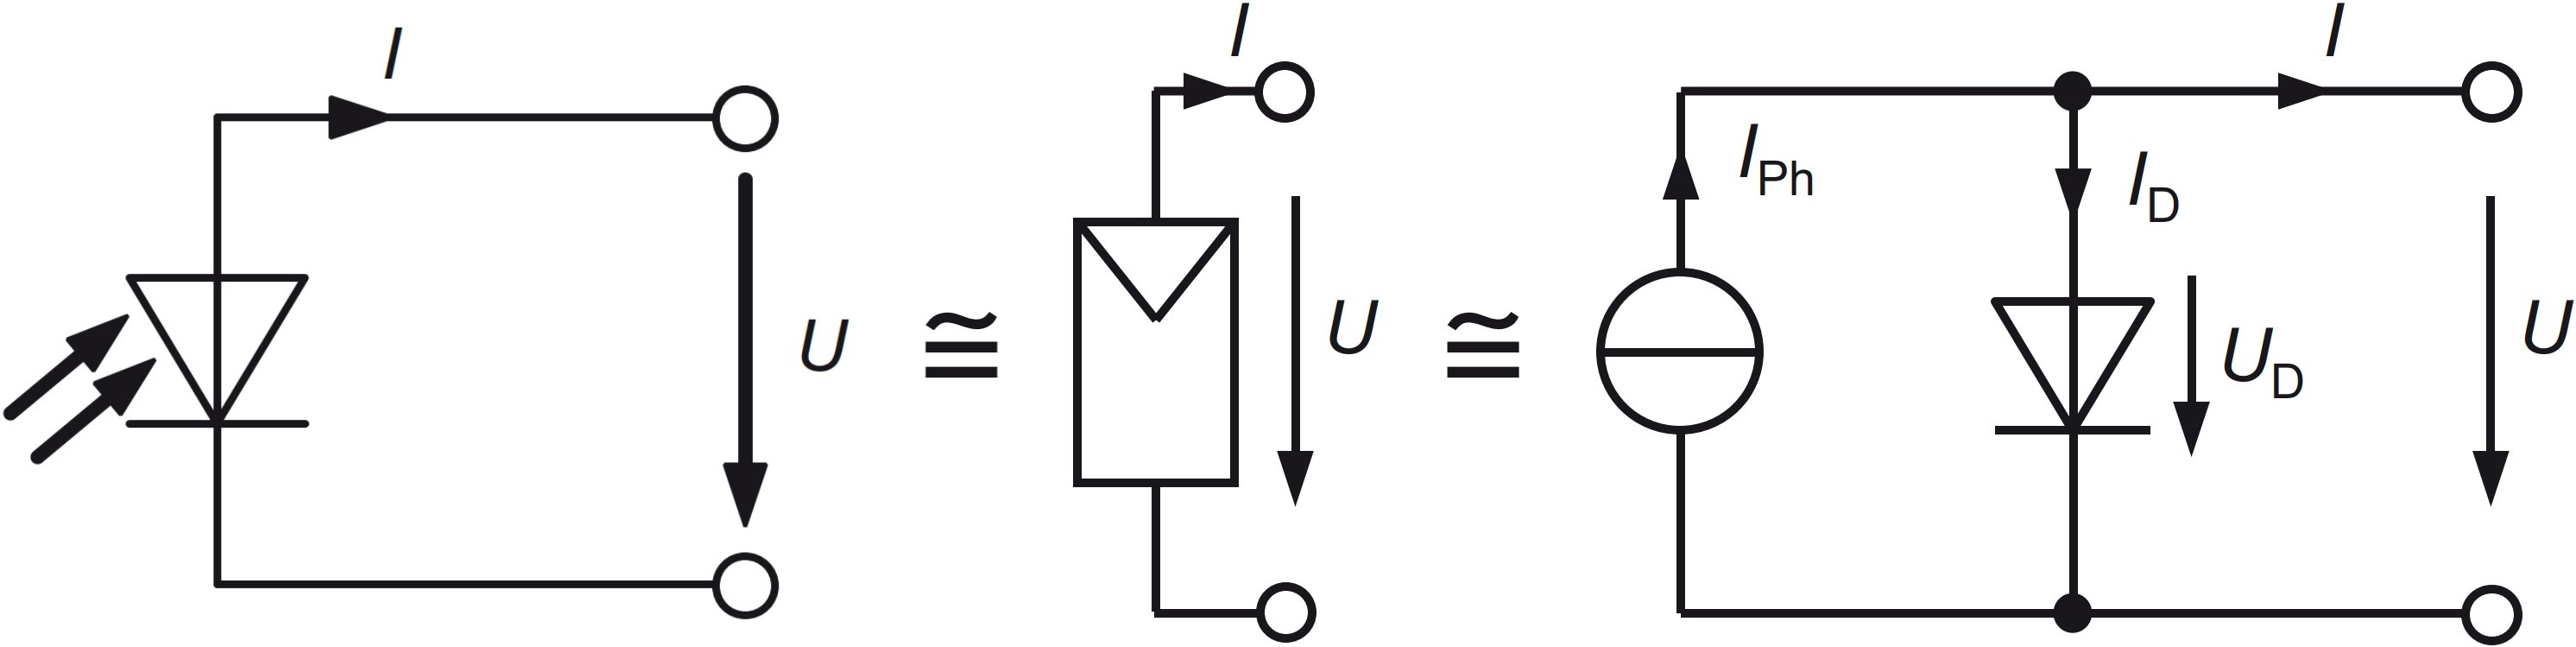
\includegraphics[width=0.8\linewidth]{images/Ersatzschaltbild_Solarzelle_1.jpg}

\vspace{0.1cm}

\begin{minipage}[t]{0.65\columnwidth}
$
\boxed{
I = I_\text{Ph} - I_\text{D} 
}
\quad
\boxed{
I = I_\text{Ph} - I_\text{S} \cdot \left( e^{\frac{U}{m \cdot U_\text{T}}} - 1 \right)
}
\quad
\boxed{
U_\text{T} = \frac{k \cdot T}{q}
}
$
\end{minipage}
\hfill
\begin{minipage}[c]{0.31\columnwidth}
    \renewcommand{\arraystretch}{1.2}
    \begin{tabular}{l}
        $k \approx 1.38 \cdot 10^{-23} \, \mathrm{\frac{J}{K}}$\\
        $q \approx 1.602 \cdot 10^{-19} \, \mathrm{C}$\\
        $m \approx 1 \dots 2$\\
    \end{tabular}
\end{minipage}

\subsubsection{Standard-Modell}

\begin{minipage}[c]{0.45\columnwidth}
    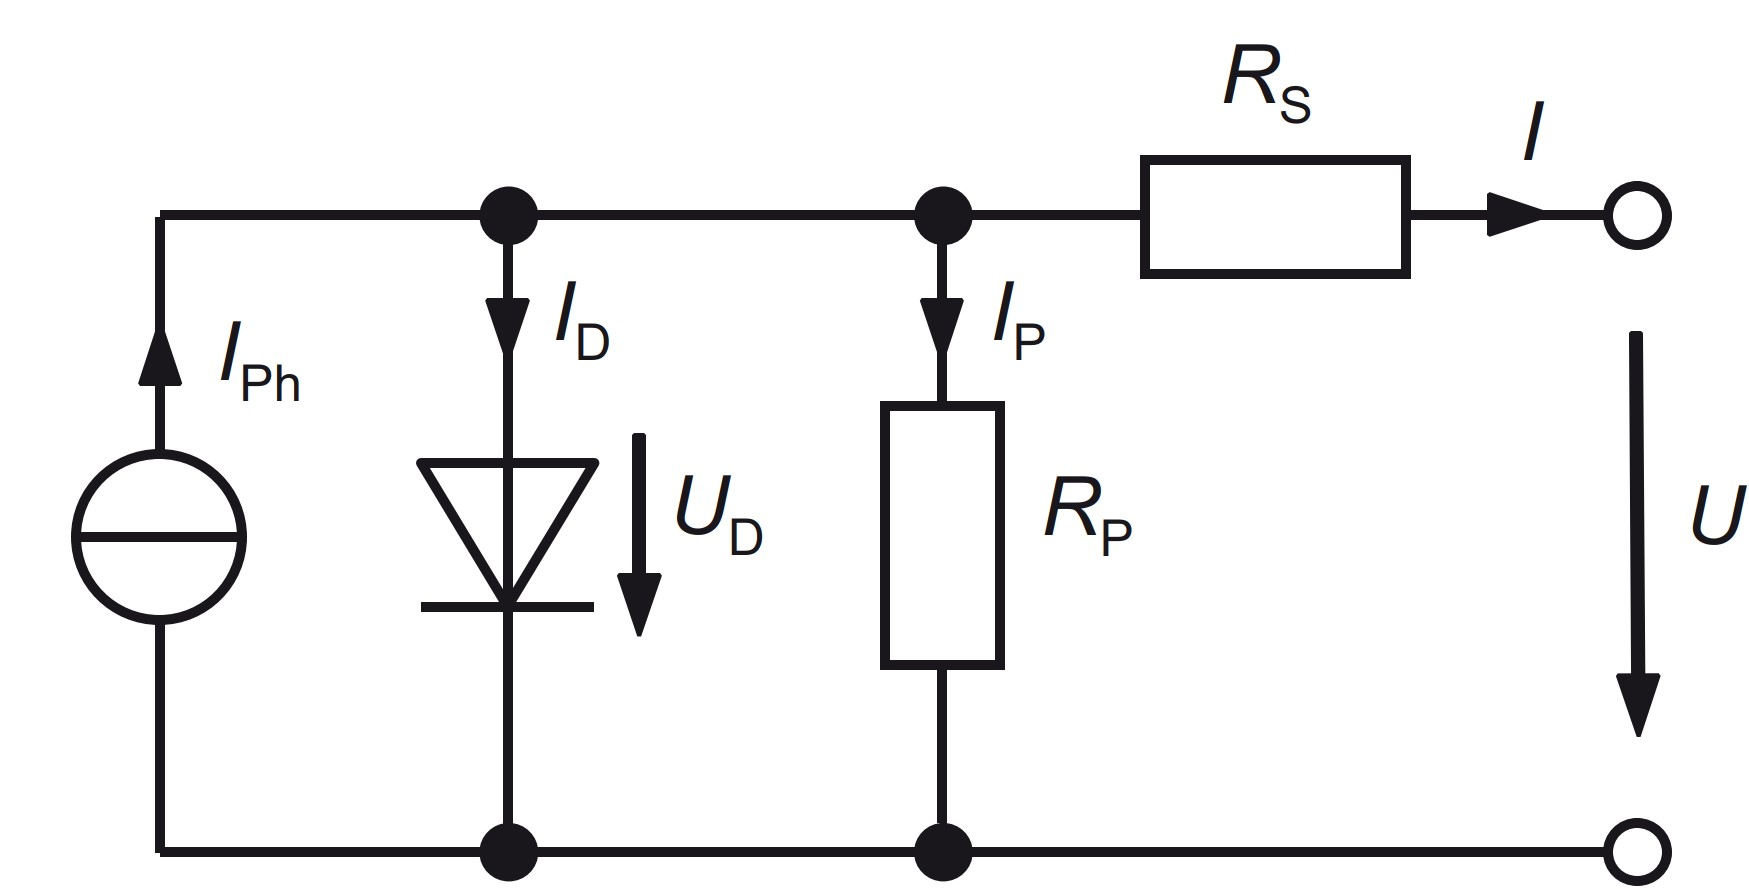
\includegraphics[width=0.98\linewidth]{images/Ersatzschaltbild_Solarzelle_2.jpg}
\end{minipage}
\hfill
\begin{minipage}[c]{0.51\columnwidth}

$
\boxed{
I = I_\text{Ph} 
- I_\text{S} \cdot \left( e^{\frac{U + I \cdot R_\text{S}}{m \cdot U_\text{T}}} - 1 \right)
- \frac{U + I \cdot R_\text{S}}{R_\text{P}}}
$

\vspace{0.1cm}

$
\boxed{I_\text{P} = \frac{U_\text{D}}{R_\text{P}} = \frac{U + I \cdot R_\text{S}}{R_\text{P}}}
$

\vspace{0.1cm}

$
\boxed{
R_\text{P} = - \left. \frac{\Delta U}{\Delta I} \right|_{U = 0}
}$
$
\boxed{
R_\text{S} = - \left. \frac{\Delta U}{\Delta I} \right|_{U = U_\text{LL}}
}
$
\end{minipage}

\vspace{0.1cm}

\begin{minipage}[t]{0.42\columnwidth}
    \renewcommand{\arraystretch}{1.2}
    \begin{tabular}{@{} l p{2.5cm} l @{}}
        $[I]$             & Solarzellenstrom \dotfill                          & $\mathrm{A}$ \\
        $[I_\text{Ph}]$   & Photostrom \dotfill                    & $\mathrm{A}$ \\
        $[I_\text{D}]$    & Diodenstrom \dotfill                                   & $\mathrm{A}$ \\
        $[I_\text{S}]$    & Sättigungsstrom \dotfill                     & $\mathrm{A}$ \\
        $[U]$             & Zellspannung \dotfill                                  & $\mathrm{V}$ \\
        $[U_\text{T}]$    & Temperaturspannung \dotfill                            & $\mathrm{V}$ \\
    \end{tabular}
\end{minipage}
\hfill
\vrule width 1pt
\hfill
\begin{minipage}[t]{0.56\columnwidth}
    \renewcommand{\arraystretch}{1.2}
    \begin{tabular}{@{} l p{3.1cm} l @{}}
        $[m]$             & Idealfaktor der Diode \dotfill & $-$ \\
        $[k]$           & Boltzmann-Konstante  \dotfill & $\mathrm{\frac{J}{K}}$ \\
        $[T]$           & Temperatur (thermodyn) \dotfill          & $\mathrm{K}$ \\
        $[q]$           & Elementarladung \dotfill & $\mathrm{C}$ \\
        $[R_\text{P}]$   & Parallelwiderstand \dotfill & $\mathrm{\Omega}$ \\
        $[R_\text{S}]$   & Serienwiderstand \dotfill & $\mathrm{\Omega}$ \\
    \end{tabular}
\end{minipage}



\columnbreak
\subsection{Spektrale Empfindlichkeit}
Die spektrale Empfindlichkeit \( S(\lambda) \) beschreibt den erzeugten Photostrom bei gegebener optischer Leistung. 



$\boxed{
S(\lambda) 
= \frac{I_{\text{Ph}}}{P_{\text{Opt}}}
}$  $\boxed{
S(\lambda) 
= \frac{\frac{Q}{\Delta t}}{\frac{W_{\text{Opt}}}{\Delta t}}
}$  $\boxed{
S(\lambda) 
= \frac{q}{h \cdot f} \cdot \eta_{\text{Ext}}
}$  $\boxed{
S(\lambda) 
= \frac{q}{h \cdot c_0} \cdot \lambda \cdot \eta_{\text{Ext}}
}$

\vspace{0.1cm}

Mit eingesetzten Konstanten ergibt sich:

\vspace{0.1cm}

$
\boxed{S(\lambda) = \frac{\lambda \cdot \eta_{\text{Ext}}}{1.24 \, \mathrm{\mu m}} \cdot \frac{\mathrm{A}}{\mathrm{W}}}
\quad
q \approx1.602 \cdot 10^{-19} \, \mathrm{Ws}
\quad
h \approx 6.6 \cdot 10^{-34} \, \mathrm{Ws^2}
\quad
c_0 \approx 3 \cdot 10^{8} \, \mathrm{\frac{m}{s}}
$

\vspace{0.1cm}

\begin{minipage}[t]{0.48\columnwidth}
    \renewcommand{\arraystretch}{1.2}
    \begin{tabular}{@{} l p{2.8cm} l @{}}
        $[S_\lambda]$       & Spektrale Empf. \dotfill          & $\frac{\mathrm{A}}{\mathrm{W}}$ \\
        $[I_\mathrm{Ph}]$   & Photostrom \dotfill               & $\mathrm{A}$ \\
        $[P_\mathrm{Opt}]$  & Optische Leist. \dotfill          & $\mathrm{W}$ \\
        $[Q]$               & Elektrische Lad. \dotfill         & $\mathrm{C}$ \\
        $[W_\mathrm{Opt}]$  & Optische Energie \dotfill         & $\mathrm{J}$ \\
        $[q]$               & Elementarladung \dotfill          & $\mathrm{C}$ 
    \end{tabular}
\end{minipage}
\hfill
\vrule width 1pt
\hfill
\begin{minipage}[t]{0.48\columnwidth}
    \renewcommand{\arraystretch}{1.2}
    \begin{tabular}{@{} l p{2.8cm} l @{}}
        $[h]$                 & Planck-Konstante \dotfill         & $\mathrm{J \cdot s}$ \\
        $[f]$                 & Frequenz \dotfill                 & $\mathrm{Hz}$ \\
        $[\eta_\mathrm{Ext}]$ & Externe Quanteneff. \dotfill      & $-$ \\
        $[c_0]$               & Lichtgeschwindigkeit \dotfill     & $\frac{\mathrm{m}}{\mathrm{s}}$\\
        $[\lambda]$           & Wellenlänge \dotfill              & $\mathrm{m}$
    \end{tabular}
\end{minipage}



\subsection{Füllfaktor und Wirkungsgrad von Solarzellen}

$
\boxed{
FF = \frac{U_{\text{MPP}} \cdot I_{\text{MPP}}}{U_{\text{L}} \cdot I_{\text{K}}} 
}$
$
\boxed{
FF = \frac{P_{\text{MPP}}}{U_{\text{L}} \cdot I_{\text{K}}}
}$
$
\boxed{
\eta = \frac{P_{\text{MPP}}}{P_{\text{opt}}} 
}$
$
\boxed{
P_{\text{MPP}} = FF \cdot U_{\mathrm{L}} \cdot I_{\mathrm{K}}
}$
$
\boxed{
P_{\text{opt}} = E \cdot A
}
$

\vspace{0.1cm}

\begin{minipage}[t]{0.44\columnwidth}
    \renewcommand{\arraystretch}{1.2}
    \begin{tabular}{@{} l p{2.4cm} l @{}}
        $[FF]$               & Füllfaktor \dotfill                            & $-$ \\
        $[\eta]$             & Wirkungsgrad \dotfill                          & $-$ \\
        $[U_{\text{MPP}}]$   & MPP-Spannung \dotfill      & $\mathrm{V}$ \\
        $[I_{\text{MPP}}]$   & MPP-Strom \dotfill         & $\mathrm{A}$ \\
        $[P_{\text{MPP}}]$   & MPP-Leistung \dotfill      & $\mathrm{W}$ \\
    \end{tabular}
\end{minipage}
\hfill
\vrule width 1pt
\hfill
\begin{minipage}[t]{0.52\columnwidth}
    \renewcommand{\arraystretch}{1.2}
    \begin{tabular}{@{} l p{3cm} l @{}}
        $[U_{\text{L}}]$     & Leerlaufspannung \dotfill                      & $\mathrm{V}$ \\
        $[I_{\text{K}}]$     & Kurzschlussstrom \dotfill                      & $\mathrm{A}$ \\
        $[E]$                & Einstrahlung \dotfill                          & $\mathrm{\frac{W}{m^2}}$ \\
        $[A]$                & Zellenfläche \dotfill                          & $\mathrm{m^2}$ \\
        $[P_{\text{opt}}]$   & Einstrahlleistung $= E \cdot A$ \dotfill & $\mathrm{W}$ \\
    \end{tabular}
\end{minipage}



\subsection{Verlustmechan. durch unpassende Energie der Photonen}

Eine fundamentale Begrenzung des Wirkungsgrads von Solarzellen ergibt sich aus dem materialabhängigen Bandabstand $\Delta W_G$ des Halbleiters. Die Wellenlänge, bei der Licht gerade noch absorbiert wird, nennen wir die \textbf{Bandlückenwellenlänge} $\lambda_G$ mit

$\boxed{\lambda_{\mathrm{G}} = \frac{h \cdot c_0}{\Delta W_G}}$
$\boxed{\Delta W_{\mathrm{G\_Krist.\ Silizium}} = 1.12e\mathrm{V}}$

\vspace{0.1cm}

\renewcommand{\arraystretch}{1.2} % Erhöht Zeilenhöhe für bessere Lesbarkeit
\begin{tabular}{@{} l p{6cm} l @{}}
    
    
\end{tabular}

\begin{minipage}[t]{0.5\columnwidth}
    \renewcommand{\arraystretch}{1.2}
    \begin{tabular}{@{} l p{3.2cm} l @{}}
        $[\lambda_{\mathrm{G}}]$       & Grenzwellenlänge Bandl    \dotfill & $\mathrm{m}$ \\
        $[h]$               & Planck-Konstante          \dotfill & $\mathrm{J \cdot s}$ \\
        $[c_0]$             & Lichtgeschwindigkeit      \dotfill & $\frac{\mathrm{m}}{\mathrm{s}}$ \\
    \end{tabular}
\end{minipage}
\hfill
\vrule width 1pt
\hfill
\begin{minipage}[t]{0.45\columnwidth}
    \renewcommand{\arraystretch}{1.2}
    \begin{tabular}{@{} l p{2.4cm} l @{}}
        $[W_{\mathrm{G}}]$             & Energie Photon            \dotfill & $\mathrm{J}$ \\
        $[\Delta W_{\mathrm{G}}]$      & Bandlücke   \dotfill & $\mathrm{J}$ \\
    \end{tabular}
\end{minipage}

\vspace{0.1cm}

\begin{minipage}[t]{0.48\columnwidth}
    \myul{\textbf{$\lambda > \lambda_G$ : Durchstrahlung}}\\
    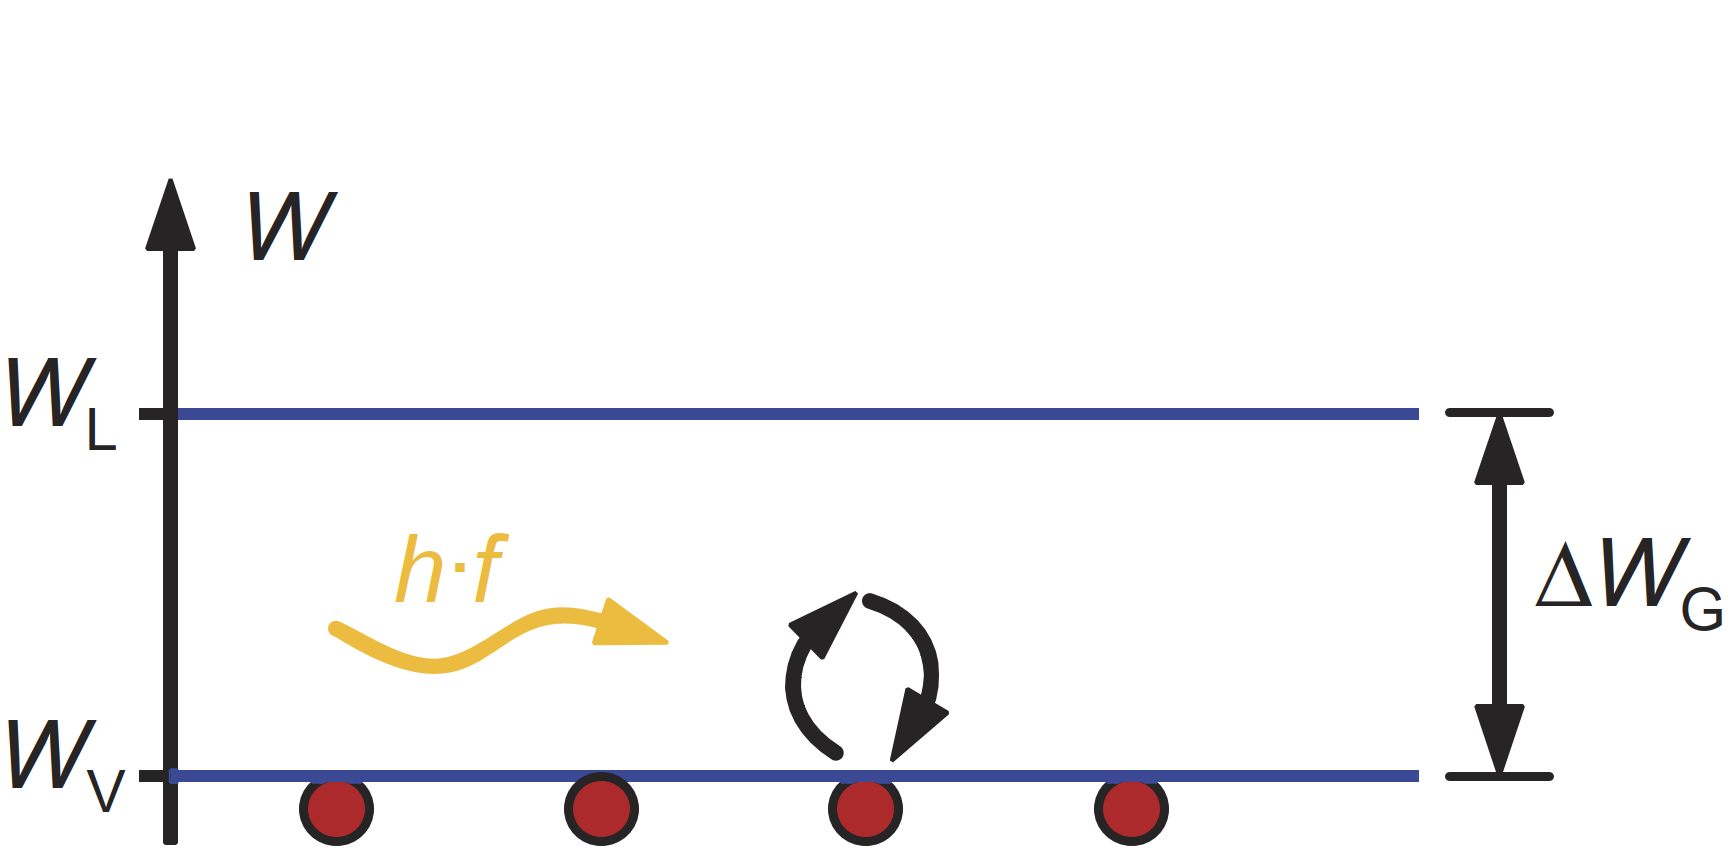
\includegraphics[width=0.9\columnwidth]{images/Spektraler_Wirkungsgrad_Durchstrahlung.png}
\end{minipage}
\hfill
\begin{minipage}[t]{0.48\columnwidth}
    \myul{\textbf{$\lambda < \lambda_G$ : Thermalisierung}}\\
    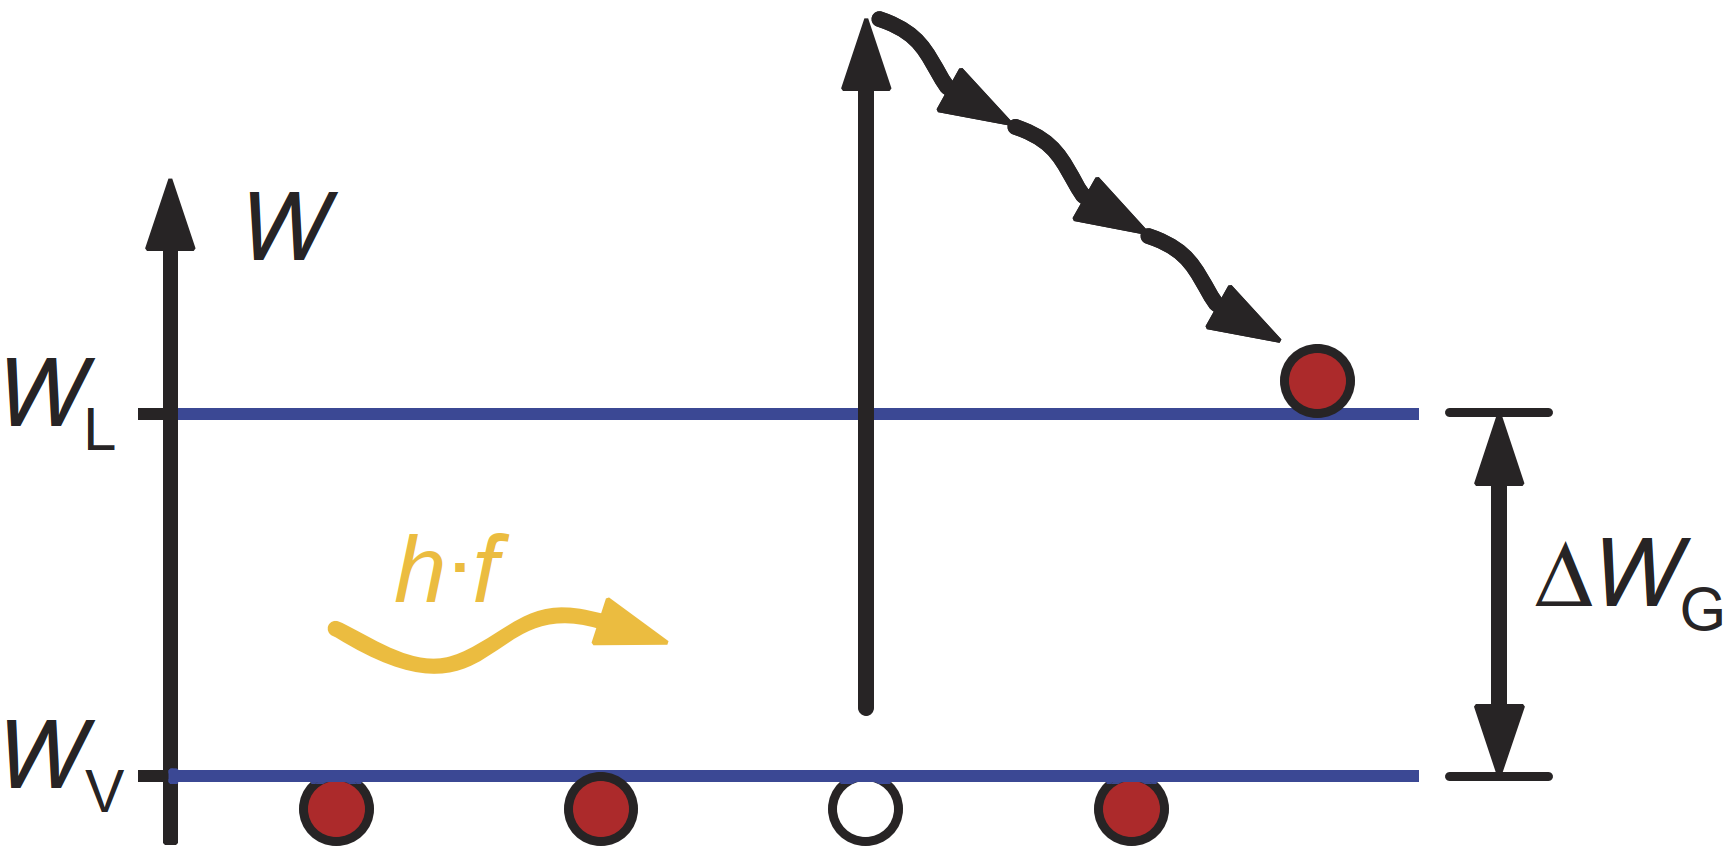
\includegraphics[width=0.9\columnwidth]{images/Spektraler_Wirkungsgrad_Thermalisierung.png}
\end{minipage}

\vspace{0.1cm}

\myul{\textbf{Durchstrahlung}} bezeichnet den Verlustmechanismus, bei dem Photonen mit zu geringer Energie die Solarzelle durchqueren, ohne absorbiert zu werden.\\
\myul{\textbf{Thermalisierung}} beschreibt den Energieverlust, bei dem Photonen mit zu hoher Energie nur einen Teil ihrer Energie an Elektronen abgeben, während die überschüssige Energie als Wärme verloren geht.



\subsection{Spektraler Wirkungsgrad $\eta_\text{S}$}

Der spektrale Wirkungsgrad gibt an, welcher Teil der einfallenden Strahlungsleistung theoretisch mit einem Halbleiter des Bandabstands \( \Delta W_G \) genutzt werden kann. Die Transmissionsverluste beschreiben den Teil des Spektrums, dessen Photonen zu energiearm sind, um die Bandlücke zu überwinden. Thermalisierungsverluste treten dagegen bei Photonen auf, die energiereicher sind als die Bandlücke. In diesem Fall kann nur ein Teil der Energie für den Halbleiter genutzt werden, der Rest wird in Wärme umgewandelt.


\vspace{0.1cm}

$
\boxed{
\eta_\text{S} = \frac{P_\text{El}}{P_\text{Opt}} = \frac{U_\text{Max} \cdot j_\text{Max}}{E}
}$
$
\boxed{
P_\text{El} = U_\text{Max} \cdot I_\text{Max} = U_\text{Max} \cdot j_\text{Max} \cdot A
}$
$
\boxed{
U_\text{Max} = \frac{\Delta W_\text{G}}{q}
}
$

\vspace{0.1cm}

\begin{minipage}[t]{0.48\columnwidth}
    \renewcommand{\arraystretch}{1.2}
    \begin{tabular}{@{} l p{2.7cm} l @{}}
        $[U_\text{Max}]$  & Maximale Spannung \dotfill        & $\mathrm{V}$ \\
        $[\Delta W_\text{G}]$  & Bandlücke \dotfill           & $\mathrm{eV}$ \\
        $[q]$             & Elementarladung \dotfill          & $\mathrm{C}$ \\
        $[P_\text{El}]$   & Elektrische Leistung \dotfill     & $\mathrm{W}$ \\
        $[I_\text{Max}]$  & Maximalstrom \dotfill             & $\mathrm{A}$ \\
    \end{tabular}
\end{minipage}
\hfill
\vrule width 1pt
\hfill
\begin{minipage}[t]{0.48\columnwidth}
    \renewcommand{\arraystretch}{1.2}
    \begin{tabular}{@{} l p{2.7cm} l @{}}
        $[j_\text{Max}]$  & Stromdichte \dotfill              & $\mathrm{A/m^2}$ \\
        $[A]$             & Zellenfläche \dotfill             & $\mathrm{m^2}$ \\
        $[P_\text{Opt}]$  & Eingestr Leistung \dotfill & $\mathrm{W}$ \\
        $[E]$             & Bestrahlungsstärke \dotfill       & $\mathrm{W/m^2}$ \\
        $[\eta_\text{S}]$ & Spektr Wirkungsgrad \dotfill  & $\mathrm{-}$ \\
    \end{tabular}
\end{minipage}



\subsection{Spektrale Verluste}
%\begin{center}
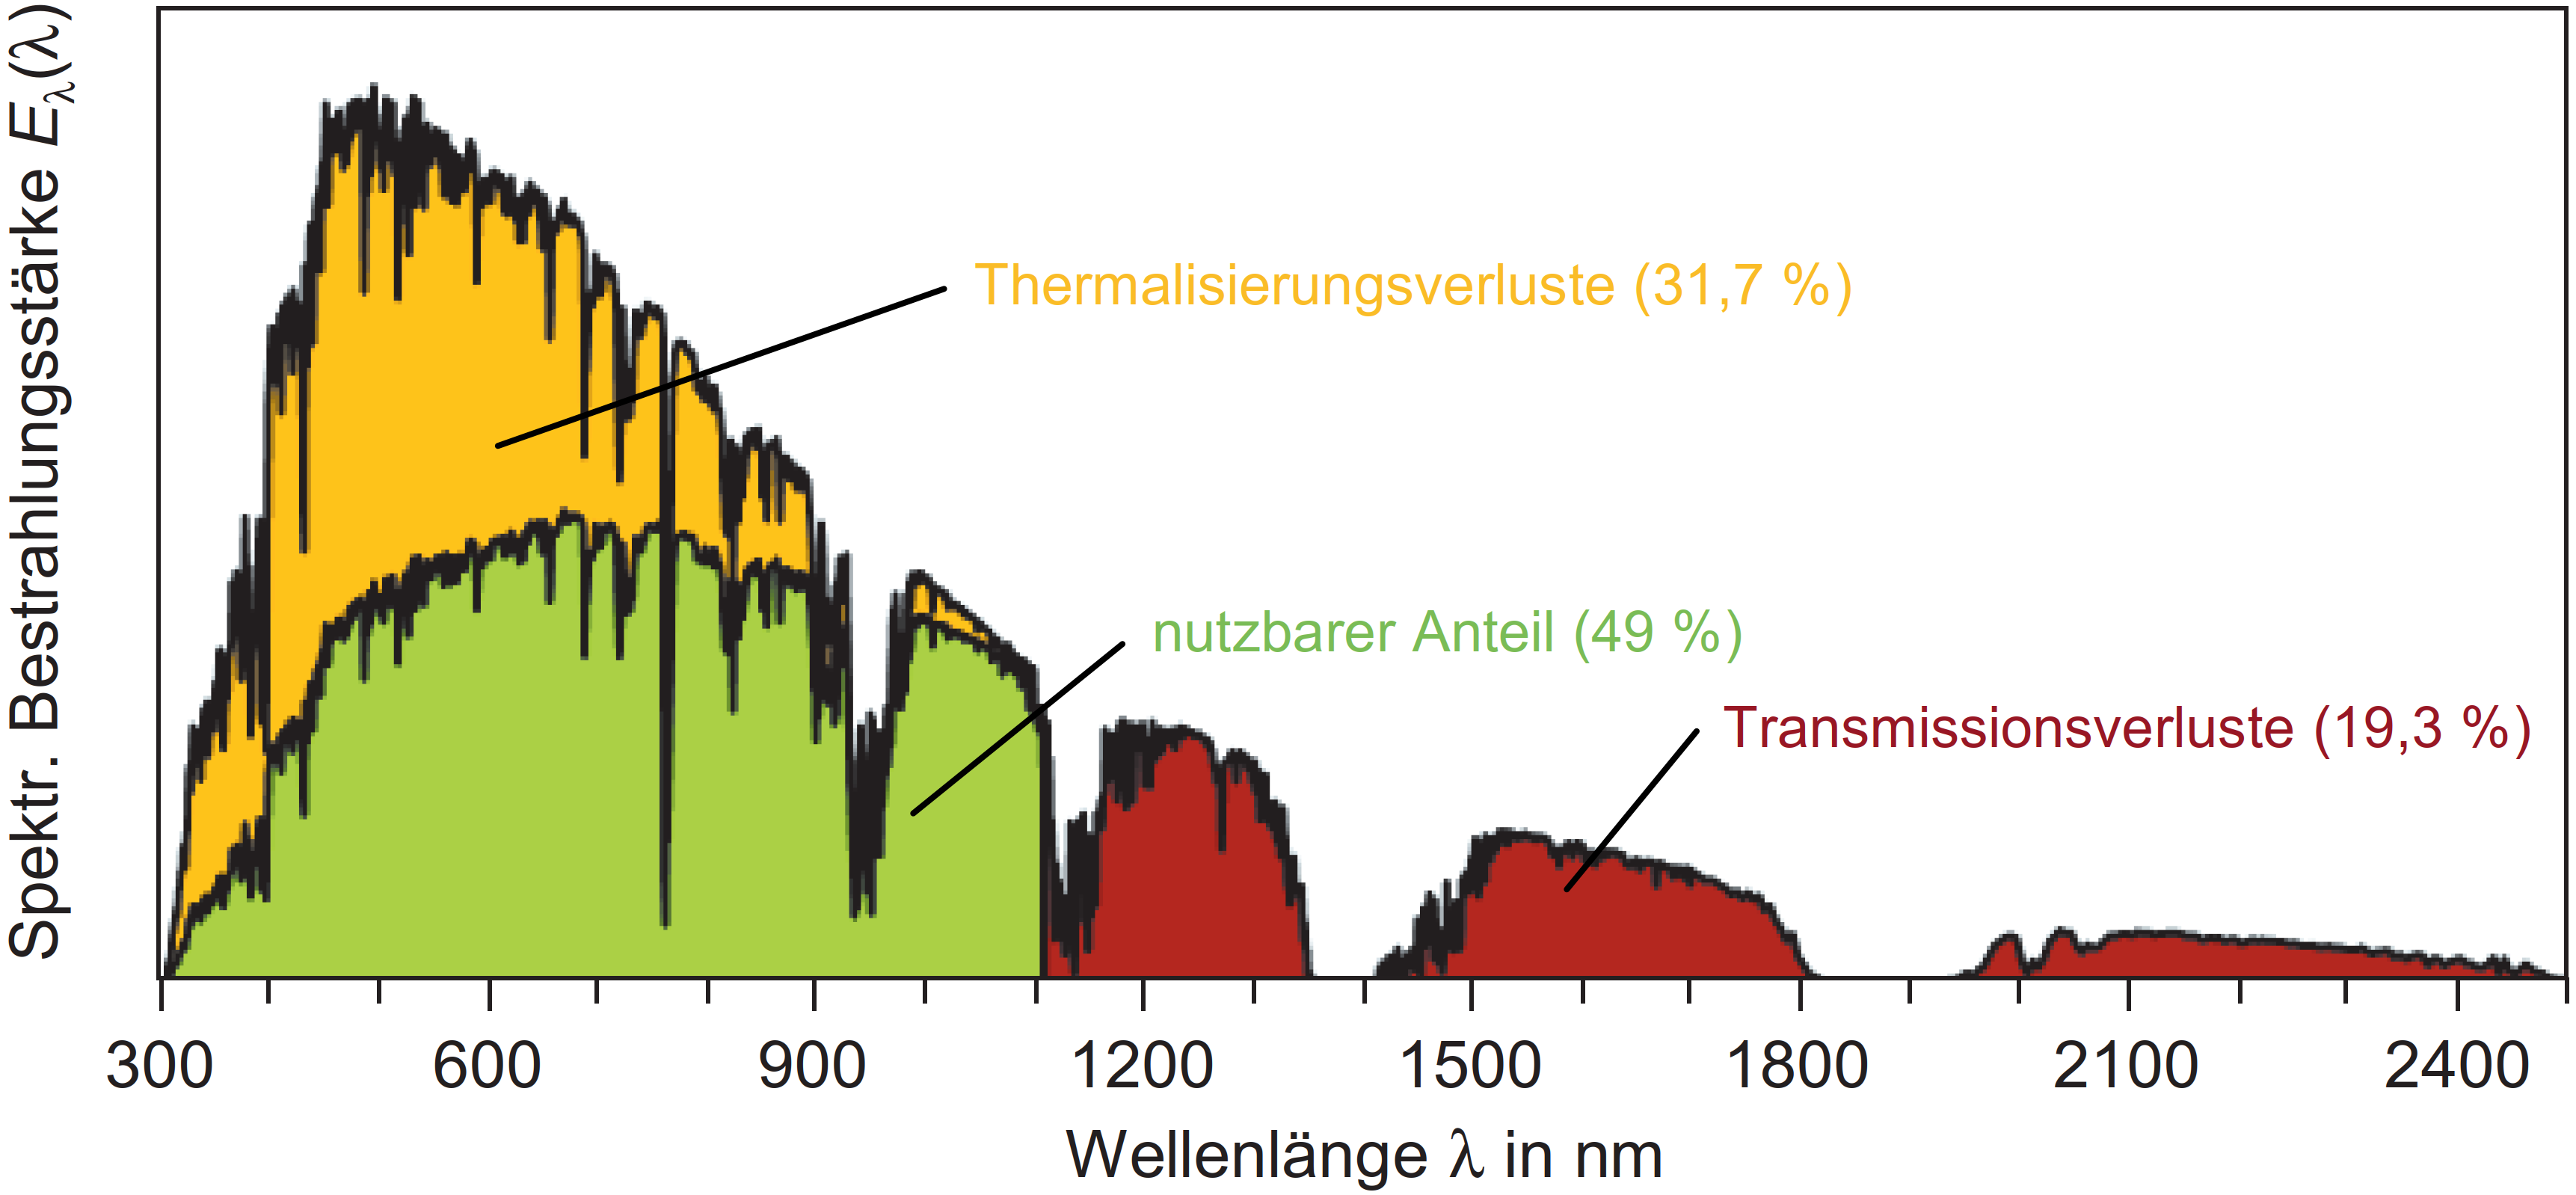
\includegraphics[width=0.8\columnwidth]{images/Spektrale_Verluste.png}
%\end{center}


\subsection{Spektrale Wirkungsgrad idealer Solarzelle}
%\textbf{Theor. max mögliche Wirkungsgr} für kristalline Siliziumsolarzelle liegt bei
%ca. $29\%$. Aktuell: $\eta_{max}$ Zelle: $27.6\%$, $\eta_{max}$ Modul: $25.4\%$, $\eta$ Typisch Module: $21-23\%$

\begin{itemize}
  \item Theoretisch maximaler Wirkungsgrad: ca. 29\,\%
  \item Aktuell erreichter maximaler Wirkungsgrad von Solarzellen: 27.6\,\%
  \item Aktuell erreichter maximaler Wirkungsgrad von Solarmodulen: 25.4\,\%
  \item Typischer Wirkungsgrad aktueller Module: ca. 21--23\,\%
\end{itemize}

%\begin{center}
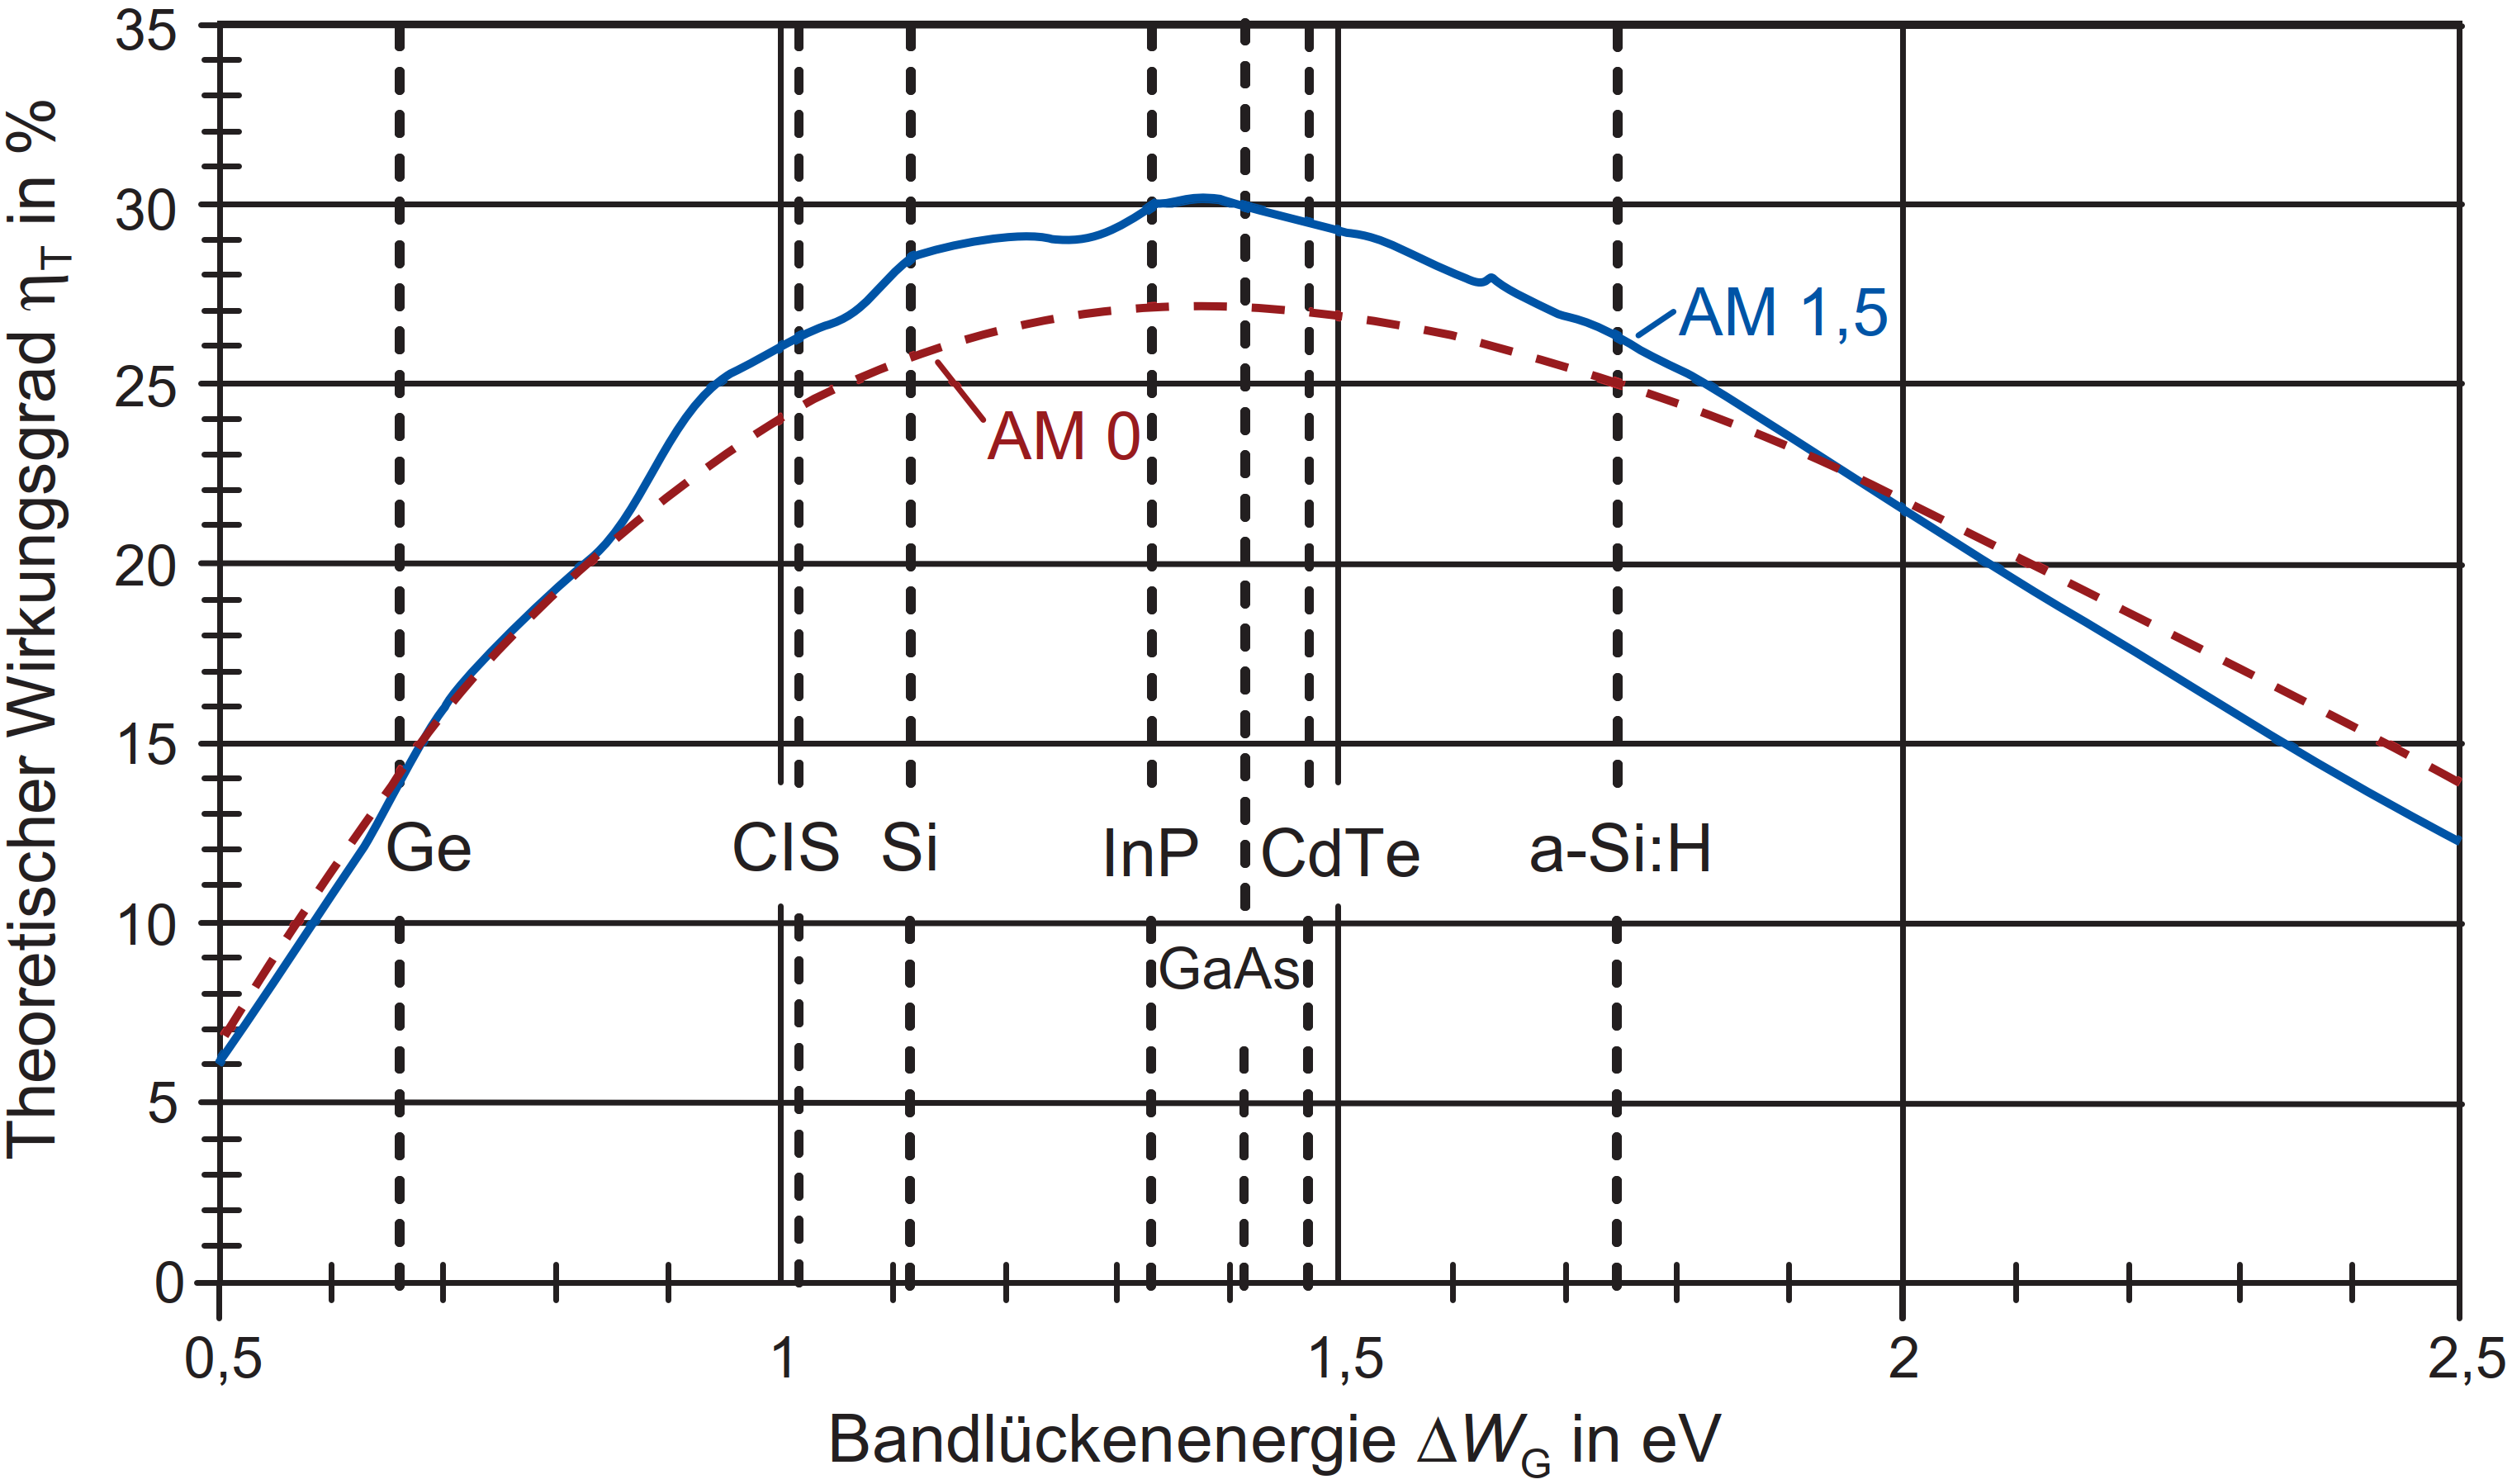
\includegraphics[width=0.8\columnwidth]{images/Spektraler_Wirkungsgrad_idealer_Solarzelle.png}
%\end{center}

\subsection{Produktionsschritte}
Für die Herstellung eines monokristallinen Solarmoduls ausgehend von Quarzsand:

\vspace{0.1cm}

\begin{enumerate}
    \item Herstellung von hochreinem Silizium (Solar-Grade-Silizium)
    \item Herstellung von monokristallinem Silizium (Ingots) im Czochralski-Verfahren
    \item Waferherstellung
    \item Solarzellenherstellung
    \item Solarmodulherstellung
\end{enumerate}

\subsection{Mehrfach- Stapelzellen}
Sie sind aus verschiedenen Halbleitermaterialien mit vers. Bandlücken aufgebaut. Es werden Photon unterschiedlicher Wellenlänge absorbiert. Damit werden höhere Wirkungsgrade erreicht (aktuell bis zu 40\%).

\subsection{Verlustfaktoren von Solarzellen: Minimierungen}

\begin{itemize}
  \item \textbf{Abschattung}: Minimierung von Kontaktfinger- und Busbarfläche, Einsatz vieler dünner Busbars, Rückseitenkontaktierung (z.B. IBC-Zelle)
  \item \textbf{Reflexion}: Antireflexbeschichtung, Texturierung der Zelloberfläche (z.B. Pyramidenstruktur)
  \item \textbf{Störstellenrekombination}: Verwendung von hochreinem Silizium (Solar-Grade), Einsatz von n-Typ Zellen
  \item \textbf{Oberflächenrekombination}: Passivierung der Oberfläche, punktuelle Kontaktierung, Durchtunnelungsschicht, Back-Surface-Field (BSF)
  \item \textbf{Transmission}: Reflektionsschicht (Oxidschicht) auf der Zellrückseite
  \item \textbf{Metall-Halbleiter-Übergang}: Lokale dotierte Schichten ($\mathrm{n^+}$ bei p-Typ, $\mathrm{p^+}$ bei n-Typ Zellen)
\end{itemize}



